Neste capítulo serão apresentados e analisados os resultados da execução do algorithmo genético, descrito na Secção~\ref{sec:gen_alg}, para a otimização do modelo de classificação, descrito na Secção~\ref{sec:neural_net}, bem como os resultados obtidos com a biblioteca PyGAD\@.

Com o auxílio da biblioteca \texttt{scikit-learn}, foi possível carregar o dataset IRIS usando a função \texttt{load\_iris}, normalizá-lo com a classe \texttt{StandardScaler}, e dividi-lo em conjuntos de treino e teste, com a função \texttt{train\_test\_split}, segundo a proporção 90/10.
Após a divisão, os conjuntos de treino e teste foram convertidos em \texttt{Tensors} do PyTorch, de modo a poderem ser utilizados pelo modelo de classificação.

\begin{listing}[!ht]
    \caption{Função para carregar os parâmetros do modelo}
    \label{alg:load_params}
    \begin{minted}[breaklines]{python}
def load_params(model: nn.Module, params: ModelParams) -> None:
    model_params = model.state_dict()
    model_params['0.weight'] = torch.FloatTensor(params[:40].reshape(10, 4))
    model_params['0.bias'] = torch.FloatTensor(params[40:50])
    model_params['2.weight'] = torch.FloatTensor(params[50:80].reshape(3, 10))
    model_params['2.bias'] = torch.FloatTensor(params[80:])
    model.load_state_dict(model_params)
    \end{minted}
\end{listing}

A seguir, foi criado um modelo de classificação, com a estrutura descrita na Secção~\ref{sec:neural_net}, com a função de ativação \texttt{ReLU} na camada oculta,
e definido o critério de erro como \texttt{CrossEntropyLoss}, dado se tratar de um problema de classificação multiclasse.

\begin{listing}[!ht]
    \caption{Função de aptidão}
    \label{alg:fitness_fn}
    \begin{minted}{python}
def fitness_fn(solution: ModelParams) -> float:
    load_params(iris_model, solution)
    with torch.no_grad():
        outputs = iris_model(X_train)
        loss = criterion(outputs, y_train)
        fitness = 1.0 / (loss.detach().item() + 1e-8)
    return fitness
    \end{minted}
\end{listing}

\begin{listing}[!ht]
    \caption{Função de `callback´ chamada em cada N gerações}
    \label{alg:on_generation}
    \begin{minted}{python}
def on_generation(generation: int, scores: list[float]) -> None:
    print(
        f"Generation: {generation:0=3} "
        f"Best fitness: {np.max(scores):.10f} "
        f"Average fitness: {np.mean(scores):.10f} "
        f"Worst fitness: {np.min(scores):.10f}"
    )
    \end{minted}
\end{listing}

Foram definidas as funções \texttt{load\_params} (Alg.~\ref{alg:load_params}), responsável por atualizar os pesos do modelo com os valores passados como argumento, a função de aptidão (Alg.~\ref{alg:fitness_fn}), que recebe como argumento um vetor de parâmetros, e retorna o inverso da função de erro, calculada com base no conjunto de treino, e a função \texttt{on\_generation}, chamada a cada geração, que imprime os valores da melhor, pior e aptidão média da população.

\begin{table}[htbp]
    \centering
    \begin{tabular}{ccc}
        \hline
        \textbf{Parâmetro}                  & \textbf{GeneticAlgorithm} & \textbf{PyGAD} \\
        \hline
        Tamanho da população                & 30                        & 10             \\
        Número de gerações                  & 600                       & 200            \\
        Intervalo de gerações               & 50                        & -              \\
        Probabilidade de mutação            & 0.05                      & -              \\
        Probabilidade de \textit{crossover} & 0.95                      & -              \\
        Probabilidade de desconexão         & $10^{-4}$                 & -              \\
        Elitismo                            & \texttt{True}             & \texttt{True}  \\
        \hline
    \end{tabular}
    \caption{Valores dos parâmetros do algoritmo genético}
    \label{tab:ga_param_values}
\end{table}

Por fim, o algoritmo genético foi instanciado com os parâmetros apresentados na Tabela~\ref{tab:ga_param_values}, que também contém os valores utilizados no algoritmo da biblioteca PyGAD\@.

\begin{figure}[htbp]
    \centering
    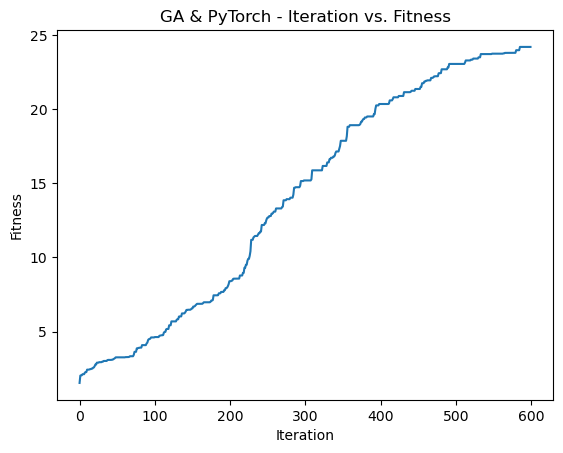
\includegraphics[width=0.65\textwidth]{images/ga_fitness}
    \caption{Evolução da aptidão da melhor solução - GeneticAlgorithm}
    \label{fig:ga_fitness}
\end{figure}

O algoritmo genético implementado com a classe \texttt{GeneticAlgorithm} foi executado durante 600 gerações, com uma população de 30 soluções.
A incorporação de elitismo provou ser eficaz, permitindo uma evolução gradual da aptidão, como é possível verificar na Fig.~\ref{fig:ga_fitness}.
Inicialmente, a aptidão apresenta um aumento prolongado, ainda que esse acelere por volta das 200 gerações.
Esse aumento torna-se menos evidente após 400 gerações, acabando por estagnar, sensivelmente, a partir de 500 iterações.

\begin{figure}[htbp]
    \centering
    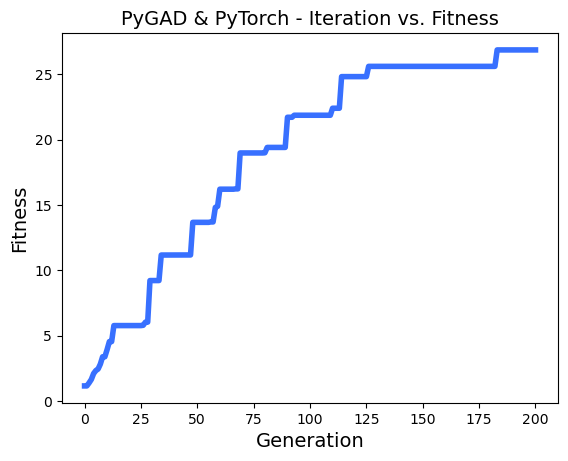
\includegraphics[width=0.65\textwidth]{images/pygad_fitness}
    \caption{Evolução da aptidão da melhor solução - PyGAD}
    \label{fig:pygad_fitness}
\end{figure}

No caso do algoritmo genético implementado com a biblioteca PyGAD, este foi executado durante 200 gerações, com uma população fixa de 10 indivíduos, ou seja, apenas $1/3$ do algoritmo original.
Dado tratar-se de uma biblioteca altamente otimizada, este foi capaz de atingir uma aptidão semelhante ao anterior em apenas 115 gerações, ainda que tenha estagnado no final da sua execução, como é evidente pela Fig.~\ref{fig:pygad_fitness}.

\begin{table}[htbp]
    \centering
    \begin{tabular}{ccc}
        \hline
        \textbf{Métricas}  & \textbf{GeneticAlgoritm} & \textbf{PyGAD} \\ \hline
        Melhor aptidão     & 24.1857                  & 26.8775        \\
        Perda de treino    & 0.0414                   & 0.0372         \\
        Acurácia de treino & 98.52\%                  & 98.52\%        \\
        Perda de teste     & 0.0112                   & 0.0120         \\
        Acurácia de teste  & 100\%                    & 100\%          \\ \hline
    \end{tabular}
    \caption{Métricas dos algoritmos}
    \label{tab:metrics}
\end{table}

Apesar do algoritmo PyGAD ter sido capaz de atingir uma aptidão final superior de 26.8775, face à aptidão do algoritmo GeneticAlgorithm de 24.1857, ambos conseguiram obter excelentes resultados na classificação das três espécies do género Iris, como é possível observar na Tabela~\ref{tab:metrics}, com uma exatidão de treino e teste de, respetivamente, 98.52\% e 100\%.